\section {Варианты расположения корней}

При рассмотрении вариантов расположения корней квадратного уравнения на промежутке или луче можно
выделить шесть основных вариантов, которые принципиально отличаются друг от друга:

%\begin {enumerate} [labelindent=\parindent, leftmargin=*, label=\Roman*., widest=IIII, align=left]
%    \item {два корня уравнения $ f(x) = 0 $ лежат внутри промежутка,}
%    \item {один корень уравнения лежит внутри промежутка,}
%    \item {внутри промежутка нет корней,}
%    \item {два корня уравнения лежат на луче,}
%    \item {один корень лежит на луче,}
%    \item {на луче нет корней.}
%\end {enumerate}

\begin {figure} [h]
    \hspace{10mm}
    \begin {minipage} [t] {0.5\linewidth}
        Вариант $I$ \\
        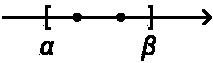
\includegraphics{images/a_dd_b.pdf}
    \end {minipage}
    \hfill
    \begin {minipage} [t] {0.5\linewidth}
        Вариант $IV$ \\
        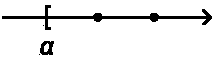
\includegraphics{images/a_dd_inf.pdf}
    \end {minipage}
    \vfill \vspace{1cm} \hspace{10mm}
    \begin {minipage} [t] {0.5\linewidth}
        Вариант $II$ \\
        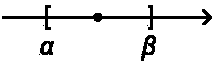
\includegraphics{images/a_d_b.pdf}
    \end {minipage}
    \hfill
    \begin {minipage} [t] {0.5\linewidth}
        Вариант $V$ \\
        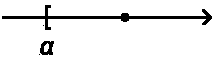
\includegraphics{images/a_d_inf.pdf}
    \end {minipage}
    \vfill \vspace{1cm} \hspace{10mm}
    \begin {minipage} [t] {0.5\linewidth}
        Вариант $III$ \\
        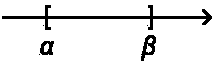
\includegraphics{images/a_b.pdf}
    \end {minipage}
    \hfill
    \begin {minipage} [t] {0.5\linewidth}
        Вариант $VI$ \\
        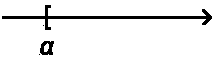
\includegraphics{images/a_inf.pdf}
    \end {minipage}
\end {figure}

Каждый вариант расположения корней подразумевает разные типы границ. От них и зависит количество
особых случаев.

\subsection {Комментарий при $D < 0$}

Такие случаи интересны только в вариантах $III$ и $VI$, а значения параметра, соответствующие им,
автоматически включаются в множество решений. Везде далее будет рассматриваться случаи с
\emph{неотрицательным дискриминантом}. Тогда вариант $VI$ "--- это практически частный случай
варианта $IV$ с тем лишь замечанием, что нужно рассматривать нахождение двух корней не на луче
$[\alpha, +\infty)$, а на луче $(-\infty, \beta=\alpha]$. Поэтому детально будут рассмотрены только
варианты $I$--$V$.


